\documentclass[11pt]{article}

\usepackage[a4paper,margin=1in]{geometry}
\usepackage{fontspec}
\usepackage{amsmath}
\usepackage{amssymb}
\usepackage{booktabs}
\usepackage{longtable}
\usepackage{array}
\usepackage{tabularx}
\usepackage{xcolor}
\usepackage{tikz}
\usetikzlibrary{shapes.geometric, arrows.meta, positioning, fit, backgrounds}
\usepackage{hyperref}
\usepackage{enumitem}
\usepackage{fancyhdr}
\usepackage{titlesec}
\usepackage{listings}
\usepackage{caption}
\usepackage{mdframed}

\definecolor{navy}{RGB}{22,44,74}
\definecolor{steel}{RGB}{70,110,142}
\definecolor{lightgray}{RGB}{245,246,248}
\definecolor{codebg}{RGB}{248,248,250}
\definecolor{riskred}{RGB}{198,40,40}
\definecolor{safegreen}{RGB}{27,94,32}

\hypersetup{
    colorlinks=true,
    linkcolor=navy,
    citecolor=navy,
    urlcolor=steel,
    pdftitle={Customer Churn Intelligence System - Data Science Design Document},
    pdfauthor={Lead ML Engineer}
}

\titleformat{\section}
  {\normalfont\Large\bfseries\color{navy}}
  {\thesection}{0.6em}{}
\titleformat{\subsection}
  {\normalfont\large\bfseries\color{steel}}
  {\thesubsection}{0.6em}{}
\titleformat{\subsubsection}
  {\normalfont\normalsize\bfseries\color{navy}}
  {\thesubsubsection}{0.6em}{}

\pagestyle{fancy}
\fancyhf{}
\fancyhead[L]{\small\textcolor{steel}{Customer Churn Intelligence System}}
\fancyhead[R]{\small\textcolor{steel}{Data Science Design Document}}
\fancyfoot[C]{\small\thepage}
\renewcommand{\headrulewidth}{0.4pt}
\renewcommand{\footrulewidth}{0pt}

\newmdenv[
  backgroundcolor=lightgray,
  linecolor=steel,
  linewidth=0.6pt,
  roundcorner=3pt,
  innerleftmargin=10pt,
  innerrightmargin=10pt,
  innertopmargin=6pt,
  innerbottommargin=6pt,
  skipabove=8pt,
  skipbelow=8pt
]{decisionbox}

\newcommand{\decision}[1]{%
\begin{decisionbox}
\textbf{\color{navy}Engineering Decision:} #1
\end{decisionbox}
}

\newcommand{\artifact}[1]{\texttt{\color{navy}#1}}

\lstset{
  basicstyle=\ttfamily\small,
  backgroundcolor=\color{codebg},
  frame=single,
  framerule=0.3pt,
  rulecolor=\color{steel},
  breaklines=true,
  columns=fullflexible,
  showstringspaces=false
}

\setlength{\parskip}{0.4em}
\setlength{\parindent}{0pt}
\setlength{\emergencystretch}{3em}
\sloppy

\title{
  \vspace{-1.5cm}
  {\Large\bfseries\color{navy} Customer Churn Intelligence System}\\[0.3em]
  {\large\color{steel} Data Science Phase --- Engineering Design Document}\\[0.2em]
  {\small\color{gray} Notebooks 01--04: EDA, Feature Engineering, Model Training, Explainability}
}
\author{}
\date{\small Prepared by the Lead ML Engineer \\ \today}

\begin{document}
\maketitle
\thispagestyle{fancy}

\begin{abstract}
\noindent
This document is the engineering design record for the Data Science phase of the Customer Churn Intelligence System, built on the IBM Telco Customer Churn dataset. It is written for an engineer joining the project after this phase has concluded, who needs to understand not just \emph{what} was implemented across the four notebooks (\texttt{01\_data\_quality\_and\_eda.ipynb}, \texttt{02\_feature\_engineering.ipynb}, \texttt{03\_model\_training.ipynb}, \texttt{04\_model\_explainability.ipynb}), but \emph{why} each decision was made, what alternatives were rejected and why, and how every artifact produced here will be consumed by the downstream ML Engineering system --- the FastAPI inference service, the batch scoring pipeline, and the business recommendation engine. Every claim in this document is grounded in the actual notebook implementations; no hypothetical or aspirational steps are described.
\end{abstract}

\tableofcontents
\newpage

% ======================================================================
\section{Business Understanding}
% ======================================================================

\subsection{The Business Problem}

Customer churn --- a subscriber terminating their telecom service --- directly erodes recurring revenue, and the economics of the telecom industry make retention structurally cheaper than acquisition: replacing a churned customer typically costs several times more than the cost of retaining them. The business objective of this project is therefore not merely to build an accurate classifier, but to build a system that lets a retention team act \emph{before} a customer leaves, with enough explanation attached to each prediction that a human can decide what action to take.

This framing matters for every subsequent engineering decision. A model that is accurate but opaque is not deployable into a retention workflow, because the retention team needs to know \emph{why} a customer is flagged in order to choose the correct intervention (a contract-upgrade incentive versus a pricing conversation versus a support outreach). This is why Section~\ref{sec:explainability} (SHAP-based explainability) is treated as a first-class deliverable of the Data Science phase rather than an optional add-on.

\subsection{Target Variable}

The modeling target is the \artifact{Churn} column, a binary label (\texttt{Yes}/\texttt{No} in the raw data). This is encoded as $1$ (churned) / $0$ (retained) in Notebook 02, Section 4, prior to the train/test split. Binary classification was the only reasonable framing here: the business question is fundamentally ``will this customer leave,'' not a multi-class or regression question, and IBM's dataset does not provide time-to-churn information that would support a survival-analysis framing.

\subsection{Why This Matters for the ML Engineering Phase}

Every artifact this phase produces is designed with the next phase already in mind:
\begin{itemize}[leftmargin=1.4em]
    \item The preprocessing logic is packaged as a \texttt{scikit-learn} \texttt{Pipeline}/\texttt{ColumnTransformer} object rather than pandas scripts, so it can be loaded, unmodified, inside a FastAPI request handler.
    \item The final model is saved as a single combined \texttt{Pipeline} (preprocessing + classifier), so the inference service has exactly one artifact to load and one \texttt{.predict\_proba()} call to make.
    \item Explainability outputs are saved as machine-readable JSON/CSV, not just notebook plots, so a recommendation engine can consume them programmatically.
\end{itemize}

This ``deploy-first'' mindset is why several choices in this document (e.g., always including a \texttt{SimpleImputer} even when no missing values remain after cleaning) look over-engineered for the current dataset but are, in fact, necessary for the system the Data Science phase is feeding into.

% ======================================================================
\section{Dataset Understanding}
% ======================================================================

The IBM Telco Customer Churn dataset contains 7,043 customer records and 21 raw columns spanning four conceptual groups: an identifier, demographic/account attributes, subscribed services, and billing information. Correctly categorizing every column was a prerequisite for building the \texttt{ColumnTransformer} in Notebook 02 --- each group receives a different transformation, so an incorrect categorization would silently corrupt the feature space.

\subsection{Identifier Columns}

\decision{\artifact{customerID} is excluded from the model's feature space entirely (Notebook 02, Section 2).}

\textbf{Problem being solved:} \artifact{customerID} is a unique string per row with no statistical relationship to churn. If passed into a one-hot encoder it would explode into thousands of meaningless dummy columns; if passed into a hashing or label encoder it would let a tree-based model memorize individual customers, producing perfect training performance that would not generalize.

\textbf{Alternative considered:} Some pipelines encode identifiers as a hashed feature for a recommendation system's join key. That is not needed here because \artifact{customerID} is retained \emph{outside} the modeling feature set (kept alongside the record in the calling application) and reattached after inference --- it never needs to enter the model to serve its purpose.

\textbf{Effect on inference:} The FastAPI/batch service will carry \artifact{customerID} through the request/response payload for CRM joins, but will strip it before calling \texttt{pipeline.transform()}. This is why the feature exclusion is recorded explicitly in \artifact{configs/feature\_columns.json} under \texttt{identifier\_columns\_excluded} rather than just implicitly dropped in code --- an inference service reading that config can validate its own input contract programmatically.

\subsection{Numerical Features}

\begin{itemize}[leftmargin=1.4em]
    \item \artifact{tenure} --- months as a customer (integer)
    \item \artifact{MonthlyCharges} --- current monthly bill (float)
    \item \artifact{TotalCharges} --- cumulative billing to date (loaded as \texttt{object}/string in the raw file --- see Section~\ref{sec:totalcharges})
\end{itemize}

These three receive median imputation followed by \texttt{StandardScaler} (Section~\ref{sec:scaling}).

\subsection{Categorical Features}

Fifteen categorical columns were identified: \artifact{gender}, \artifact{Partner}, \artifact{Dependents}, \artifact{PhoneService}, \artifact{MultipleLines}, \artifact{InternetService}, \artifact{OnlineSecurity}, \artifact{OnlineBackup}, \artifact{DeviceProtection}, \artifact{TechSupport}, \artifact{StreamingTV}, \artifact{StreamingMovies}, \artifact{Contract}, \artifact{PaperlessBilling}, \artifact{PaymentMethod}. None of these have a natural ordering (e.g., \artifact{InternetService} values \texttt{DSL}/\texttt{Fiber optic}/\texttt{No} are categorical, not ordinal), which is the deciding factor in choosing one-hot over ordinal encoding (Section~\ref{sec:onehot}).

A structural detail surfaced during EDA (Notebook 01, Section 4.6) is that six of these columns (\artifact{OnlineSecurity}, \artifact{OnlineBackup}, \artifact{DeviceProtection}, \artifact{TechSupport}, \artifact{StreamingTV}, \artifact{StreamingMovies}) contain a third category, \texttt{"No internet service"}, that is fully determined by \artifact{InternetService == 'No'}. This redundancy was deliberately \emph{not} collapsed in feature engineering --- see Section~\ref{sec:onehot} for the reasoning.

\subsection{Binary Passthrough Feature}

\artifact{SeniorCitizen} is stored in the raw data as an integer 0/1 flag, not a string. It is semantically categorical (a demographic binary), but because it arrives pre-encoded, it is routed to its own lightweight pipeline branch (imputation only, no scaling, no one-hot) rather than being forced through the categorical or numerical branches. This is a deliberate categorization decision, not an oversight: one-hot encoding an already-binary 0/1 column would double its width for zero informational gain, and scaling it would be harmless but unnecessary. Keeping it as a distinct group makes the \texttt{ColumnTransformer} definition self-documenting --- anyone reading Notebook 02 can see at a glance which columns needed which treatment and why.

\subsection{Why This Categorization Was Necessary}

The entire \texttt{ColumnTransformer} in Notebook 02 (Section 9) is built directly from these three lists (\texttt{numerical\_features}, \texttt{categorical\_features}, \texttt{binary\_passthrough\_features}). An assertion in the notebook (\texttt{assert set(numerical\_features + binary\_passthrough\_features + categorical\_features) == set(X.columns)}) enforces that every column is accounted for exactly once --- this guards against the single most common feature-engineering bug in production pipelines: a column silently falling through \texttt{ColumnTransformer}'s default \texttt{remainder} behavior and either being dropped unintentionally or passed through untransformed.

% ======================================================================
\section{Data Quality Assessment}
% ======================================================================

\subsection{Missing Value Analysis}

Standard pandas null detection (\texttt{df.isnull().sum()}) found zero missing values across all 21 columns (Notebook 01, Section 4.3). This result was intentionally \emph{not} taken at face value. \artifact{TotalCharges} was loaded as an \texttt{object} dtype rather than a numeric type, which is a classic signal of embedded non-numeric characters that pandas' null detector cannot see. A targeted check (\texttt{(df['TotalCharges'].astype(str).str.strip() == '')}) found 11 blank-string entries.

\subsection{The TotalCharges Type Conversion}
\label{sec:totalcharges}

\decision{Blank \artifact{TotalCharges} strings are coerced to numeric via \texttt{pd.to\_numeric(..., errors='coerce')} and the resulting nulls are filled with $0.0$, but only after verifying every affected row has \texttt{tenure == 0} (Notebook 02, Section 3).}

\textbf{Problem being solved:} A string-typed numeric column cannot be scaled, cannot be fed to any \texttt{scikit-learn} numeric transformer, and will silently crash --- or worse, be silently misinterpreted --- at inference time if the type mismatch is not resolved upstream.

\textbf{Why this specific fill value was chosen:} All 11 blank rows correspond to customers with \texttt{tenure == 0} --- i.e., brand-new customers who have not yet received a bill. This is not missing data in the statistical sense; it is a deterministic consequence of the business process (\artifact{TotalCharges} $\approx$ \artifact{tenure} $\times$ \artifact{MonthlyCharges}, so zero tenure implies zero total charges). The notebook encodes an explicit \texttt{assert} verifying this precondition before applying the fill, rather than blindly imputing:
\begin{lstlisting}
assert (df.loc[zero_tenure_mask, 'tenure'] == 0).all()
df['TotalCharges'] = df['TotalCharges'].fillna(0.0)
\end{lstlisting}

\textbf{Alternatives considered and rejected:}
\begin{itemize}[leftmargin=1.4em]
    \item \emph{Statistical imputation (mean/median)} --- would have introduced a fabricated value with no business grounding, when the true value (0) is actually knowable with certainty.
    \item \emph{Row deletion} --- would have discarded 11 legitimate customer records for a problem that has a clean, correct fix; also risky in production, where deleting rows silently changes batch inference output cardinality against the input.
    \item \emph{Leaving as \texttt{NaN} and letting the pipeline's \texttt{SimpleImputer} handle it downstream} --- rejected because the assertion-verified business rule is more precise than a generic \texttt{median} imputer would be, and because the type coercion has to happen before the train/test split regardless (dtype correction is not a leakage-sensitive operation, unlike scaling or the imputer's learned statistic).
\end{itemize}

\textbf{What happens if this step is skipped:} Any downstream numeric transformer (\texttt{StandardScaler}, the eventual XGBoost split logic) would either raise a \texttt{ValueError} on non-numeric input or silently coerce the whole column to \texttt{NaN}, corrupting 100\% of the feature rather than the 0.16\% actually affected.

\textbf{Effect on inference:} The \texttt{SimpleImputer(strategy='median')} inside the numerical branch of the production \texttt{ColumnTransformer} (Section~\ref{sec:columntransformer}) is the safety net for this exact failure mode at inference time --- a live record arriving with a blank/malformed \artifact{TotalCharges} will be median-imputed automatically rather than crashing the API. The explicit business-rule fill in Notebook 02 handles the \emph{training}-time cleaning; the pipeline's built-in imputer handles the same class of problem robustly in \emph{production}.

\subsection{Duplicate Analysis}

No fully duplicated rows and no duplicate \artifact{customerID} values were found (Notebook 01, Section 4.4). No deduplication logic was required in the pipeline. This was verified rather than assumed, since silent duplicate customers would have inflated the effective weight of those customers during model training.

\subsection{Invalid Data Detection}

Notebook 01, Section 4.5 checked for negative tenures, negative charges, and non-binary values in \artifact{SeniorCitizen} --- none were found. The implied relationship \artifact{tenure} $\times$ \artifact{MonthlyCharges} $\approx$ \artifact{TotalCharges} was also spot-checked; observed deviations were attributed to historical price changes/promotions rather than data corruption, and required no correction.

\subsection{Outlier Analysis}

An IQR-based outlier check (Notebook 01, Section 8) found no meaningful outliers in any of the three numerical features --- all values are naturally bounded by business logic (tenure in months, charges in dollars). \textbf{No outlier removal or clipping was applied.} This is a deliberate absence of action, documented so a future engineer does not assume outlier handling was overlooked; it was investigated and found unnecessary.

\subsection{Summary of Data Quality Findings}

\begin{center}
\begin{tabularx}{\textwidth}{@{}l X X@{}}
\toprule
\textbf{Check} & \textbf{Finding} & \textbf{Action Taken} \\
\midrule
Missing values (standard) & 0 detected by pandas & None needed \\
Missing values (targeted) & 11 blank \artifact{TotalCharges} strings, all \texttt{tenure==0} & Numeric coercion + rule-based fill to 0.0 \\
Duplicates & 0 duplicate rows / IDs & None needed \\
Invalid values & None found & None needed \\
Outliers & None found (IQR method) & None needed \\
\bottomrule
\end{tabularx}
\end{center}

% ======================================================================
\section{Exploratory Data Analysis}
% ======================================================================

The EDA in Notebook 01 was structured around business questions, not around producing plots for their own sake. Each analysis below directly influenced a later decision in feature engineering, modeling, or explainability.

\subsection{Business Question: Is the target balanced enough to use accuracy as the primary metric?}

The target distribution (Notebook 01, Section 5) showed approximately 73\% retained / 27\% churned --- confirmed precisely in Notebook 02/03 as a 26.5\% churn rate in both the train and test splits. This moderate imbalance directly caused two downstream decisions: (1) every model in Notebook 03 was trained with \texttt{class\_weight='balanced'} (or XGBoost's \texttt{scale\_pos\_weight}), and (2) accuracy was explicitly excluded from the model-selection criterion in favor of ROC-AUC, precision, recall, and F1 evaluated together.

\subsection{Business Question: Which customers are most at risk, and does the model's later behavior make business sense?}

\begin{itemize}[leftmargin=1.4em]
    \item \textbf{Tenure:} Churn is concentrated in the first months of a customer relationship (Notebook 01, Section 6). This directly foreshadowed \artifact{tenure} emerging as the single strongest SHAP driver in Notebook 04, and grounded the ``first 90 days retention program'' business recommendation.
    \item \textbf{Contract type:} Month-to-month customers churn at a dramatically higher rate than one-/two-year contract holders (Notebook 01, Section 7). This became the top global SHAP feature (\artifact{Contract\_Month-to-month}, mean $|\text{SHAP}| = 0.676$, the largest of any feature) in Notebook 04 --- a direct confirmation that the model learned a pattern the business already suspected, which materially increases stakeholder trust in the model.
    \item \textbf{Pricing:} Churners pay higher \artifact{MonthlyCharges} on average, and this effect compounds with contract flexibility (Notebook 01, Section 10) --- within every contract type, churners pay more, but the gap is largest for month-to-month customers.
    \item \textbf{Payment method and billing style:} Electronic check payment and paperless billing correlate with elevated churn (Notebook 01, Section 7), interpreted as behavioral proxies for a less ``locked-in'' customer relationship rather than causal levers --- a distinction carried through explicitly into the Model Limitations section of Notebook 04.
    \item \textbf{Service add-ons:} Customers lacking \artifact{OnlineSecurity} and \artifact{TechSupport} churn more --- this insight directly shaped the business recommendation to use these add-ons as retention tools, not just upsell revenue.
\end{itemize}

\subsection{Business Question: Is there a multicollinearity risk that affects model choice?}

The correlation analysis (Notebook 01, Section 9) found \artifact{tenure} and \artifact{TotalCharges} to be highly correlated, since the latter accumulates from the former. This is a real concern for a linear model (Logistic Regression coefficients become unstable/hard to interpret under collinearity) but a non-issue for tree-based models (Random Forest, XGBoost split on whichever correlated feature reduces impurity most, without coefficient instability). This observation is why Logistic Regression was retained in the model comparison as a baseline/interpretability reference, but was not expected -- and did not turn out -- to be the top performer.

\subsection{How EDA Findings Fed Forward}

\begin{center}
\begin{tabularx}{\textwidth}{@{}l X@{}}
\toprule
\textbf{EDA Finding} & \textbf{Downstream Consequence} \\
\midrule
27\% churn rate (moderate imbalance) & \texttt{class\_weight='balanced'} / \texttt{scale\_pos\_weight} in all models; ROC-AUC-first model selection \\
\artifact{TotalCharges} type + blank strings & Explicit numeric coercion \& rule-based fill in Notebook 02 \\
No outliers & No clipping/winsorization step added to the pipeline \\
No ordinal categories & One-hot encoding chosen over ordinal/label encoding \\
Redundant ``No internet service'' categories & Left un-collapsed; handled naturally by one-hot + \texttt{handle\_unknown='ignore'} \\
tenure/Contract dominance & Directly corroborated by SHAP global importance in Notebook 04, reinforcing model trust \\
\bottomrule
\end{tabularx}
\end{center}

% ======================================================================
\section{Feature Engineering}
% ======================================================================

This is the largest section of this document because Notebook 02 produces the artifacts that everything downstream --- model training, explainability, and eventually the FastAPI service --- depends on directly.

\subsection{Design Principle: Everything Must Be Serializable}

\decision{All cleaning and transformation logic that must run identically at both training and inference time is implemented as \texttt{scikit-learn} \texttt{Pipeline}/\texttt{ColumnTransformer} objects, not standalone pandas code.}

Hand-written pandas transformations (e.g., \texttt{df['x'].fillna(...)} called ad hoc) cannot be shipped to a FastAPI service safely, because there is nothing to serialize --- the logic lives only in notebook cells. By contrast, an object built from \texttt{scikit-learn} transformers can be fit once and pickled (\texttt{joblib.dump}), then loaded identically inside the notebook, inside a unit test, and inside the production API, guaranteeing training/serving parity. The only exception to this rule in Notebook 02 is the \artifact{TotalCharges} type coercion and zero-fill (Section~\ref{sec:totalcharges}), which is deliberately implemented as an explicit, auditable, assertion-guarded pandas operation \emph{before} the pipeline, precisely because it encodes a business rule that benefits from being visible and asserted rather than buried inside a generic imputer.

\subsection{Median Imputation for Numerical Features}

\textbf{Purpose:} Guard the numerical branch (\artifact{tenure}, \artifact{MonthlyCharges}, \artifact{TotalCharges}) against missing values at inference time.

\textbf{Reason for selection:} Median is robust to skew and outliers relative to mean imputation. Although Notebook 01's outlier analysis found no current outliers, this is a forward-looking safeguard --- live production data is not guaranteed to remain as clean as the static training snapshot.

\textbf{Alternatives considered:} Mean imputation (rejected --- more sensitive to any future skew or data entry errors); KNN or iterative imputation (rejected as unnecessary complexity/latency cost for three low-missingness numerical columns at inference time, where a single API request cannot wait on a KNN search over historical data).

\textbf{Advantages:} Simple, fast, robust, fully serializable, deterministic.

\textbf{Disadvantages:} Does not use any cross-feature information (unlike KNN imputation); on the current dataset this is a non-issue since no numerical missingness remains after the Section~\ref{sec:totalcharges} fix, meaning the imputer executes as a no-op during training. It exists purely as inference-time protection.

\textbf{Effect on downstream inference:} If a live customer record has a null/missing numeric field, the API will substitute the training-set median for that field automatically rather than raising an exception. This is deliberately a defensive measure, not a modeling choice --- it changes production reliability more than it changes model accuracy.

\subsection{Most-Frequent Imputation for Categorical Features}

\textbf{Purpose:} Analogous inference-time protection for the fifteen categorical columns.

\textbf{Reason for selection:} Mode imputation is the standard robust default for categorical data with no natural numeric ordering; it never invents a category that does not exist in the training distribution.

\textbf{Alternatives considered:} A dedicated \texttt{"Missing"} category (rejected --- would require a corresponding code path anywhere the feature is later interpreted, e.g., in SHAP explanations, adding interpretive complexity for no clear benefit versus mode imputation on this dataset).

\textbf{Effect on downstream inference:} Identical rationale to the numerical case --- a live record with a missing categorical field is filled with that field's most common training-set value rather than crashing the request.

\subsection{StandardScaler for Numerical Features}
\label{sec:scaling}

\textbf{Purpose:} Rescale \artifact{tenure}, \artifact{MonthlyCharges}, \artifact{TotalCharges} to zero mean / unit variance.

\textbf{Reason for selection:} Logistic Regression's gradient-based optimizer converges faster and produces directly comparable coefficients when features are on a common scale; without scaling, \artifact{TotalCharges} (range up to several thousand) would dominate the loss surface and any regularization penalty relative to, say, \artifact{tenure} (range 0--72).

\textbf{Why it is safe for the tree-based models too:} Random Forest and XGBoost split on threshold comparisons within a single feature at a time, so scaling is a no-op for them --- it changes neither their splits nor their predictions. This is precisely why a \emph{single shared preprocessing pipeline} could serve all four model families in Notebook 03 without per-model branching logic.

\textbf{Alternatives considered:} \texttt{MinMaxScaler} (rejected --- more sensitive to any future outliers appearing in production data, since it is anchored to observed min/max rather than distributional mean/std); no scaling at all (rejected --- would have made the Logistic Regression baseline non-competitive and its coefficients uninterpretable).

\textbf{Effect on downstream inference:} The scaler's mean/std are learned once from the training split and frozen inside \artifact{preprocessor.pkl}. Every future inference request is transformed using these frozen statistics, never recomputed --- this is essential for reproducibility, since recomputing scaling statistics per batch would make a single customer's predicted probability depend on which other customers happened to be in the same batch request.

\subsection{OneHotEncoder for Categorical Features}
\label{sec:onehot}

\textbf{Purpose:} Convert the fifteen unordered categorical columns into a numeric representation usable by every candidate model.

\textbf{Reason for selection:} None of the fifteen categorical features have a natural order (Section 2.3), which rules out ordinal encoding. One-hot encoding is the standard, model-agnostic choice that avoids implying a false ordinal relationship (e.g., encoding \artifact{InternetService} as \texttt{DSL=0, Fiber optic=1, No=2} would falsely imply \texttt{No < DSL < Fiber optic} to a linear model).

\textbf{Handling of the redundant ``No internet service'' category:} As noted in Section 2.3, six columns contain a category value that is fully determined by \artifact{InternetService == 'No'}. This redundancy was \emph{deliberately not collapsed}. One-hot encoding absorbs it naturally as its own indicator column at negligible cost given the dataset's modest cardinality, and collapsing it would require custom, non-standard, harder-to-maintain logic for a modeling benefit that does not materialize at this feature-set size. This is an explicit trade-off in favor of pipeline simplicity over marginal dimensionality reduction.

\textbf{The \texttt{handle\_unknown='ignore'} setting:} This is one of the most operationally important lines in the entire notebook. Without it, the encoder raises an exception the first time it encounters a category value it did not see during training (for example, if the business introduces a new \artifact{PaymentMethod} option after the model is deployed). With it, an unseen category is encoded as all-zeros for that feature's indicator columns, and the request proceeds instead of crashing the API. \textbf{What would happen if this were skipped:} a single new payment method rolled out by the business, with no corresponding model retrain, would take down the entire inference endpoint for every request carrying that value --- a production outage caused entirely by a preprocessing default, not a modeling failure.

\textbf{Alternatives considered:} Target/mean encoding (rejected --- introduces target leakage risk if not implemented with careful out-of-fold logic, and adds a stateful lookup that must itself be versioned and validated at inference time; not justified given the modest cardinality here); ordinal/label encoding (rejected per above).

\textbf{Effect on downstream inference:} The fitted \texttt{OneHotEncoder}'s learned category vocabulary is frozen inside \artifact{preprocessor.pkl}. The full list of resulting output column names is also persisted in \artifact{configs/feature\_columns.json} under \texttt{transformed\_feature\_names}, so any downstream consumer (e.g., the SHAP explainer in Notebook 04, or a future monitoring job) can align feature-level outputs to human-readable names without re-deriving them.

\subsection{Binary Passthrough Handling}

\textbf{Purpose:} Pass \artifact{SeniorCitizen} through with only defensive imputation, no encoding or scaling.

\textbf{Reason for selection:} The column already arrives as a clean 0/1 integer flag; one-hot encoding it would double its width (two indicator columns) for a feature that is already minimal and correctly typed, and scaling a binary flag provides no benefit to any of the four candidate models.

\textbf{Effect on downstream inference:} This column passes through the pipeline essentially unchanged (aside from imputation protection), keeping the transformed feature space smaller and the SHAP explanations for this feature directly interpretable as ``0 vs.\ 1'' rather than as a scaled or encoded quantity.

\subsection{The ColumnTransformer}
\label{sec:columntransformer}

\begin{lstlisting}
preprocessor = ColumnTransformer(
    transformers=[
        ('num', numerical_transformer, numerical_features),
        ('cat', categorical_transformer, categorical_features),
        ('bin', binary_transformer, binary_passthrough_features),
    ],
    remainder='drop',
    verbose_feature_names_out=False
)
\end{lstlisting}

\textbf{Purpose:} Apply the three branch-specific transformations (Sections 5.2--5.5) to their respective column subsets within a single, fittable, serializable object.

\textbf{Why \texttt{remainder='drop'} matters:} This setting means any column not explicitly assigned to one of the three branches is silently dropped rather than passed through untransformed. Combined with the coverage assertion in Section 2.5, this makes the feature contract airtight --- there is no code path by which an un-reviewed column could leak into the model.

\textbf{Alternatives considered:} Building three separate, manually-orchestrated pipelines and concatenating their outputs with \texttt{numpy.hstack} (rejected --- \texttt{ColumnTransformer} already solves this problem, is the standard idiom, and --- critically --- is itself directly serializable via \texttt{joblib}, whereas a hand-rolled concatenation function is not).

\subsection{The Full Pipeline Object}

The \texttt{ColumnTransformer} above is the \artifact{preprocessor}. In Notebook 03, it is composed with a classifier into a single \texttt{Pipeline([('preprocessor', ...), ('classifier', ...)])} object per candidate model. This composition is what allows the entire system --- cleaning, encoding, scaling, and prediction --- to be invoked with one \texttt{.predict\_proba()} call on a raw, uncleaned customer record, which is exactly the contract the FastAPI service will rely on.

\subsection{Feature Selection: A Deliberate Non-Decision}

No automated feature selection (recursive feature elimination, variance thresholding, correlation-based pruning) was applied in Notebook 02. This is documented as a deliberate decision, not an omission, for three reasons argued in the notebook:

\begin{enumerate}[leftmargin=1.4em]
    \item \textbf{Low dimensionality.} After one-hot encoding, the feature space is on the order of 30--45 columns --- far from the regime where tree ensembles or L2-regularized linear models struggle with the curse of dimensionality.
    \item \textbf{Implicit regularization already exists.} Logistic Regression's default L2 penalty and the tree ensembles' split-importance mechanics perform a soft, learned form of feature selection during training itself.
    \item \textbf{Explainability requires the full feature set.} SHAP analysis in Notebook 04 is most informative when every original business feature (e.g., \artifact{Contract}, \artifact{PaymentMethod}) remains visible to the model, rather than being pruned away before the model ever sees it --- pre-filtering would have made several of the Section 11 business insights impossible to surface.
\end{enumerate}

Feature importance is instead examined \emph{post hoc}, after training, via SHAP --- which is a more defensible sequence than a blind pre-filter, since it lets the data (not an assumption) determine what mattered.

% ======================================================================
\section{Train/Test Split}
% ======================================================================

\subsection{Why the Split Was Performed}

An 80/20 stratified split (\texttt{stratify=y}, \texttt{random\_state=42}) was applied in Notebook 02, Section 5, \emph{before} any transformer was fit. Stratification preserves the $\approx$26.5\% churn rate in both the training set (26.54\%) and test set (26.54\%) --- verified numerically in the notebook output --- which prevents an unlucky random split from producing a test set with a meaningfully different class balance than production traffic is expected to have.

\subsection{Why Preprocessing Was Fitted Only on Training Data}

\decision{\texttt{preprocessor.fit(X\_train)} is called exactly once, on the training split only; the test split is only ever \texttt{.transform()}'d, never used to (re-)fit any statistic.}

\textbf{Problem being solved:} If the \texttt{StandardScaler}'s mean/std or the \texttt{OneHotEncoder}'s category vocabulary were fit on the full dataset (train + test combined), information from the test set --- which is supposed to simulate unseen future data --- would leak into the numbers used to transform the training set. The model would then be implicitly ``aware'' of statistics derived from data it is being evaluated against, inflating the apparent test performance relative to what the model will actually achieve on truly unseen production data.

\textbf{How leakage was avoided in this specific implementation:} The fit/transform separation is enforced structurally, not just by convention --- \texttt{preprocessor.fit(X\_train)} is called once, and \texttt{X\_test\_transformed = preprocessor.transform(X\_test)} is the only operation ever applied to the test features. The round-trip sanity check at the end of Notebook 02 (reloading \artifact{preprocessor.pkl} and re-transforming a test sample) additionally verifies that the persisted artifact behaves identically to the in-memory fitted object, closing the loop between ``what was fit'' and ``what gets shipped.''

\textbf{A subtler leakage risk, and how it was handled in Notebook 03:} Cross-validation and grid search (Section~\ref{sec:hyperparam}) do \emph{not} reuse the single already-fitted \artifact{preprocessor.pkl}. Instead, each candidate model is wrapped in its own fresh \texttt{Pipeline([('preprocessor', clone(preprocessor)), ('classifier', model)])}, so that every cross-validation fold refits its own preprocessing statistics on that fold's training portion only. Reusing the one pipeline fitted on the full training set across CV folds would have leaked each fold's held-out portion's statistics into the scaler/encoder fit for every other fold containing it in the full training set. The \emph{final} deployed \artifact{model.pkl}, in contrast, is refit with the canonical full-training-set \artifact{preprocessor.pkl} equivalent, matching what Notebook 02 already produced, since at deployment time there is no longer a need to simulate a held-out fold.

\textbf{Why this matters in production ML systems generally:} Data leakage between train/test (or train/validation folds) is one of the most common causes of a model that looks excellent in a notebook and then underperforms materially once deployed against genuinely new customers. A leaked evaluation number is worse than a slightly lower, honest one, because it produces false confidence in a model that will disappoint the business after the resources have already been committed to deploying it.

% ======================================================================
\section{Model Development}
% ======================================================================

Four model families were trained and compared in Notebook 03, each wrapped in the shared preprocessing pipeline.

\subsection{Logistic Regression}
\textbf{Why included:} Serves as an interpretable, fast-training baseline; its coefficients (post-scaling) give a directly interpretable linear view of feature effects, useful as a sanity check against the more complex models' SHAP explanations.\\
\textbf{Strengths:} Fast, interpretable, well-calibrated probabilities, low variance.\\
\textbf{Weaknesses:} Assumes a linear (log-odds) relationship between features and target; sensitive to the \artifact{tenure}/\artifact{TotalCharges} multicollinearity noted in EDA; cannot capture feature interactions without manual engineering.\\
\textbf{Configuration:} \texttt{class\_weight='balanced'}, \texttt{max\_iter=2000} (increased from the default to guarantee convergence given the one-hot expanded feature width).

\subsection{Decision Tree}
\textbf{Why included:} A single-tree reference point --- useful for establishing whether ensembling (Random Forest) actually adds value over this dataset, and for a maximally interpretable (if less accurate) fallback.\\
\textbf{Strengths:} Naturally handles non-linear relationships and interactions; requires no scaling; trivially interpretable as a decision path.\\
\textbf{Weaknesses:} High variance --- a single tree easily overfits without depth constraints; this is exactly what was observed (see Section~\ref{sec:modelselection}: Decision Tree had the lowest test ROC-AUC of the four, at 0.8346, despite the highest raw recall).\\
\textbf{Configuration:} \texttt{class\_weight='balanced'}; depth/leaf-size were tuned via grid search (Section~\ref{sec:hyperparam}) rather than left at defaults, specifically to control this overfitting tendency.

\subsection{Random Forest}
\textbf{Why included:} An ensembling approach that directly addresses the single Decision Tree's variance problem by averaging many de-correlated trees.\\
\textbf{Strengths:} Handles non-linearities and interactions natively; robust to outliers and irrelevant features; requires no scaling; competitive accuracy with tree-based ensembles.\\
\textbf{Weaknesses:} Larger memory footprint and slower inference than a single linear model or single tree; less directly interpretable than Logistic Regression (though SHAP restores interpretability post hoc, see Section~\ref{sec:explainability}).\\
\textbf{Configuration:} \texttt{class\_weight='balanced'}, \texttt{n\_jobs=-1} for parallelized training; \texttt{n\_estimators}, \texttt{max\_depth}, and \texttt{min\_samples\_leaf} tuned via grid search.

\subsection{XGBoost}
\textbf{Why included:} Gradient boosting typically achieves the strongest tabular-data performance among tree-based methods on datasets of this size and structure, and was included as the ``performance ceiling'' candidate.\\
\textbf{Strengths:} Sequential error-correcting boosting often captures subtler patterns than bagged trees; built-in handling of class imbalance via \texttt{scale\_pos\_weight}; pairs efficiently and exactly with SHAP's \texttt{TreeExplainer}.\\
\textbf{Weaknesses:} More hyperparameters to tune than Random Forest (learning rate, depth, number of estimators all interact); more prone to overfitting if learning rate/depth are not controlled, which is why the grid search explicitly searched conservative depths (3, 5) and learning rates (0.05, 0.1) rather than only high-capacity configurations.\\
\textbf{Configuration:} \texttt{scale\_pos\_weight} computed directly from the observed train-set class ratio ($\approx$2.77), \texttt{eval\_metric='logloss'}.

\subsection{Why Model Comparison Was Necessary}

No single model family is guaranteed to be optimal for a given tabular dataset's specific structure (linear-separable signal vs.\ interaction-heavy signal, feature cardinality, sample size). Committing to one architecture without comparison risks leaving material performance on the table, and --- just as importantly for this project's later phases --- risks choosing a model that is harder to explain (Section~\ref{sec:explainability}) than a comparably accurate alternative would have been. Cross-validated comparison, followed by held-out test evaluation, is the standard, defensible way to make this choice auditable.

\subsection{Final Model Selection}
\label{sec:modelselection}

\begin{center}
\begin{tabular}{lccccc}
\toprule
\textbf{Model} & \textbf{Accuracy} & \textbf{Precision} & \textbf{Recall} & \textbf{F1} & \textbf{ROC-AUC} \\
\midrule
\textbf{XGBoost (selected)} & 0.7424 & 0.5095 & 0.7914 & 0.6199 & \textbf{0.8443} \\
Random Forest & 0.7466 & 0.5147 & 0.7941 & 0.6246 & 0.8420 \\
Logistic Regression & 0.7388 & 0.5052 & 0.7834 & 0.6143 & 0.8407 \\
Decision Tree & 0.7346 & 0.5000 & 0.8209 & 0.6215 & 0.8346 \\
\bottomrule
\end{tabular}
\captionof{table}{Held-out test set results, all four tuned models (Notebook 03, Section 5).}
\end{center}

\textbf{XGBoost was selected} on the basis of the highest held-out ROC-AUC (0.8443), combined with a cross-validated ROC-AUC (0.8471) close enough to its test-set score to indicate the grid search did not overfit the validation folds. Note that Random Forest's test ROC-AUC (0.8420) and other metrics are extremely close to XGBoost's --- this is reported honestly in this document rather than overstated, because the practical difference between the top two candidates on this dataset is small. XGBoost was preferred as the tiebreak specifically because it pairs with SHAP's exact \texttt{TreeExplainer} just as efficiently as Random Forest does, so the explainability requirement did not itself distinguish between the two; the ROC-AUC edge was the deciding quantitative factor. The selection logic in the notebook is implemented programmatically (\texttt{best\_model\_name = test\_results\_df.iloc[0]['Model']}), so this document's claim about which model was chosen is derived from, and will remain synchronized with, the actual code path rather than being hard-coded prose.

% ======================================================================
\section{Hyperparameter Optimization}
\label{sec:hyperparam}
% ======================================================================

\subsection{Cross-Validation Strategy}

A 5-fold \texttt{StratifiedKFold} (\texttt{shuffle=True}, \texttt{random\_state=42}) was used throughout Notebook 03, for both the initial baseline comparison and the grid searches. Stratification is essential here for the same reason it mattered for the train/test split (Section 6.1): with a 26.5\% positive rate, a non-stratified fold could easily land at, say, 18\% or 35\% churn by chance, distorting that fold's evaluation of precision/recall.

\subsection{GridSearchCV}

Each of the four candidates was tuned via \texttt{GridSearchCV} scoring on \texttt{roc\_auc}, chosen because ROC-AUC is also the primary model-selection metric (Section~\ref{sec:evaluation}) --- the tuning objective and the selection objective are deliberately kept identical, so the ``best'' hyperparameters found are best with respect to the same criterion the final model choice is judged on.

\begin{center}
\begin{tabularx}{\textwidth}{@{}l X X@{}}
\toprule
\textbf{Model} & \textbf{Grid Searched} & \textbf{Selected (best)} \\
\midrule
Logistic Regression & \texttt{C} $\in \{0.01, 0.1, 1.0, 10.0\}$ & (regularization strength selected by CV) \\
Random Forest & \texttt{n\_estimators} $\in \{200, 400\}$, \texttt{max\_depth} $\in \{6, 10, \text{None}\}$, \texttt{min\_samples\_leaf} $\in \{1, 5\}$ & (best combination per CV) \\
XGBoost & \texttt{n\_estimators} $\in \{200, 400\}$, \texttt{max\_depth} $\in \{3, 5\}$, \texttt{learning\_rate} $\in \{0.05, 0.1\}$ & \texttt{n\_estimators=200}, \texttt{max\_depth=3}, \texttt{learning\_rate=0.05} \\
Decision Tree & \texttt{max\_depth} $\in \{4,6,8,10\}$, \texttt{min\_samples\_leaf} $\in \{1,5,10\}$ & (best combination per CV) \\
\bottomrule
\end{tabularx}
\captionof{table}{Hyperparameter grids searched per model family.}
\end{center}

\subsection{Interpreting the Selected XGBoost Hyperparameters}

The final selected configuration --- \texttt{max\_depth=3}, \texttt{learning\_rate=0.05}, \texttt{n\_estimators=200} --- is a conservative, shallow-tree, low-learning-rate combination. This is directly consistent with the EDA finding that this dataset's signal is dominated by a small number of strong, largely monotonic features (\artifact{tenure}, \artifact{Contract}) rather than deep, high-order interactions: a shallow-tree ensemble captures that kind of signal well without the added variance risk of deeper trees. The grid search choosing the shallowest depth option (3, not 5) and the more conservative of the two learning rates (0.05, not 0.1) is itself evidence against the risk of an overfit final model.

\subsection{Why Hyperparameter Tuning Was Necessary at All}

Default hyperparameters are tuned by library authors for a wide, generic range of datasets and are not guaranteed to be optimal for this specific feature space, sample size, and class balance. Skipping this step risks leaving a materially weaker model in production purely because, e.g., XGBoost's default \texttt{max\_depth} or Random Forest's default \texttt{n\_estimators} happened not to suit this particular problem --- an easily avoidable and easily auditable gap.

% ======================================================================
\section{Model Evaluation}
\label{sec:evaluation}
% ======================================================================

\subsection{Metrics Used, and Why Each Matters for Churn Prediction Specifically}

\begin{itemize}[leftmargin=1.4em]
    \item \textbf{Accuracy (0.7424 for the selected model):} Reported for completeness, but explicitly \emph{not} used for model selection. With a 26.5\% positive rate, a trivial model that always predicts ``No Churn'' would already score $\approx$73.5\% accuracy while providing zero business value --- accuracy alone cannot distinguish a useful model from a useless one on an imbalanced target like this.
    \item \textbf{Precision (0.5095, churn class):} Answers ``of the customers we flagged as likely to churn, what fraction actually churn?'' This matters because every flagged customer typically triggers a retention cost (a discount offer, an outreach call) --- low precision means wasted retention spend on customers who were never going to leave.
    \item \textbf{Recall (0.7914, churn class):} Answers ``of the customers who actually churn, what fraction did we catch?'' This is the metric most directly tied to the business's core motivation (Section 1): a missed churner (false negative) costs the full customer lifetime value, which is typically far more expensive than a wasted retention offer (false positive). This asymmetry is why recall was used as an explicit secondary tiebreaker in model selection, alongside ROC-AUC.
    \item \textbf{F1 (0.6199):} The harmonic mean of precision and recall, useful as a single-number summary when the two are in tension, but --- consistent with the reasoning above --- was not the primary selection criterion, since it implicitly weights precision and recall equally when the business cost asymmetry argues for weighting recall somewhat higher.
    \item \textbf{ROC-AUC (0.8443, the primary selection criterion):} Measures ranking quality across every possible decision threshold, not just the default 0.5 cutoff. This was chosen as the primary criterion specifically because the model's probability output --- not a hard yes/no --- is what will be exposed to the downstream business recommendation engine (Section~\ref{sec:mle}), which is expected to bucket customers into risk tiers (e.g., high/medium/low) using thresholds chosen later based on retention-offer economics, not the default 0.5 used for the classification-report metrics in this notebook. A model with strong ROC-AUC will rank customers sensibly regardless of exactly where those business thresholds end up being set.
\end{itemize}

\subsection{Confusion Matrix and ROC Curve}

Confusion matrices (Notebook 03, Section 6) and ROC curves (Section 7) were generated for all four tuned models for visual side-by-side comparison. The ROC curve comparison in particular makes the near-tie between XGBoost and Random Forest visually apparent, corroborating the numeric closeness reported in Table~\ref{sec:modelselection}'s comparison (both curves sit almost on top of each other for most of the false-positive-rate range).

\subsection{Full Classification Report (Selected Model)}

\begin{center}
\begin{tabular}{lccc}
\toprule
\textbf{Class} & \textbf{Precision} & \textbf{Recall} & \textbf{F1-score} \\
\midrule
No Churn (support 1035) & 0.9058 & 0.7246 & 0.8052 \\
Churn (support 374) & 0.5095 & 0.7914 & 0.6199 \\
\midrule
Macro avg & 0.7076 & 0.7580 & 0.7125 \\
Weighted avg & 0.8006 & 0.7424 & 0.7560 \\
\bottomrule
\end{tabular}
\end{center}

The stark asymmetry between the two classes' precision (0.9058 for No-Churn vs.\ 0.5095 for Churn) is expected and acceptable given the class imbalance and the \texttt{class\_weight}/\texttt{scale\_pos\_weight} adjustment: the model has been deliberately biased toward catching more churners (high recall on the minority class, 0.7914) at the cost of more false-positive churn flags on the majority class. This is the correct trade-off given the cost asymmetry discussed above, and it is a direct, intentional consequence of the class-imbalance handling strategy chosen in Section 7, not an unexamined side effect.

% ======================================================================
\section{Model Serialization}
% ======================================================================

This section documents the four production artifacts generated across Notebooks 02 and 03. These are the actual hand-off deliverables of the Data Science phase --- everything before this point exists to justify and produce these four files correctly.

\subsection{\texttt{preprocessor.pkl}}
\textbf{Contents:} The fitted \texttt{ColumnTransformer} object (Section~\ref{sec:columntransformer}) --- frozen \texttt{StandardScaler} mean/std, frozen \texttt{OneHotEncoder} category vocabulary, and both \texttt{SimpleImputer} statistics --- all fit exclusively on the training split.\\
\textbf{How it will be consumed downstream:} Loaded directly inside the FastAPI service (and the batch scoring job) via \texttt{joblib.load}, then called as \texttt{preprocessor.transform(raw\_customer\_record)} to convert an incoming raw request into the exact numeric feature vector the model expects.\\
\textbf{Why saved separately from the model:} Keeping the preprocessor as its own artifact (rather than only inside the combined \texttt{model.pkl}) allows it to be reused independently --- for instance, by the SHAP explainer in Notebook 04, which needs the transformed feature matrix and feature names but operates on the classifier object directly, not the full pipeline's \texttt{.predict()} interface.

\subsection{\texttt{model.pkl}}
\textbf{Contents:} The full, final \texttt{Pipeline([('preprocessor', ...), ('classifier', XGBClassifier(...))])} object --- i.e., the fitted preprocessor \emph{and} the tuned XGBoost classifier composed into one callable object.\\
\textbf{How it will be consumed downstream:} This is the single artifact the FastAPI inference endpoint loads to serve predictions: one \texttt{joblib.load}, one \texttt{.predict\_proba(raw\_record)[:, 1]} call, no separate preprocessing step required by the calling code. The batch scoring job uses the identical call pattern on a dataframe of many records at once.\\
\textbf{Why saved separately from \texttt{preprocessor.pkl}:} The combined pipeline is the deployment artifact; the standalone preprocessor is the explainability/debugging artifact. Shipping only the combined pipeline would have made it awkward for Notebook 04 to access the transformed feature matrix independently of a full prediction call.

\subsection{\texttt{metrics.json}}
\textbf{Contents:} Selected model name, selection criterion (documented in plain text inside the JSON itself), full test-set metrics (accuracy/precision/recall/F1/ROC-AUC), the winning cross-validated ROC-AUC, the selected hyperparameters, the full four-model comparison table, the complete \texttt{classification\_report} (per-class and averaged), and the train/test churn-rate class balance.\\
\textbf{How it will be consumed downstream:} This is the evaluation baseline for production model monitoring --- once the FastAPI service is live and scoring real traffic, its ongoing recall/precision/ROC-AUC (once true labels become available, e.g., 30/60/90 days later when actual churn/retention outcomes are known) can be compared against these numbers to detect model drift or degradation. It also feeds a model card for stakeholder/compliance review without needing to re-open the notebooks.\\
\textbf{Why saved separately:} A human- and machine-readable JSON is far easier to diff across model versions, feed into a CI pipeline's regression check, or display on a monitoring dashboard than metrics embedded only in notebook output cells.

\subsection{\texttt{feature\_columns.json}}
\textbf{Contents:} The raw input column contract (\texttt{raw\_input\_columns}), the three feature-group lists (numerical/categorical/binary), the full list of transformed (post-encoding) feature names, the excluded identifier columns, the target column and its Yes/No $\to$ 1/0 mapping, and the random seed/test-size used for the split.\\
\textbf{How it will be consumed downstream:} The FastAPI service can validate an incoming request's JSON payload against \texttt{raw\_input\_columns} \emph{before} calling the model, returning a clear 422 validation error for a malformed request rather than an opaque pipeline exception. The \texttt{transformed\_feature\_names} list is what lets the SHAP explainer (and any future monitoring/logging of feature-level statistics) label its output meaningfully rather than working with anonymous array indices.\\
\textbf{Why saved separately:} This is metadata \emph{about} the preprocessor, not the preprocessor's fitted state itself --- keeping it in a plain, human-readable JSON (rather than requiring a Python/joblib environment just to inspect what columns the model expects) makes it usable by non-Python tooling too (e.g., a request-validation layer written in a different language, or simple documentation generation).

\subsection{Why These Four Artifacts Are Kept Separate Rather Than Bundled}

Each artifact has a distinct consumer and a distinct update cadence: \artifact{preprocessor.pkl} and \artifact{model.pkl} are binary, environment-coupled objects that change only when the pipeline or model is retrained; \artifact{metrics.json} and \artifact{feature\_columns.json} are lightweight, human-readable metadata that other systems (monitoring dashboards, API validation layers, documentation generators) need to read \emph{without} requiring a Python/joblib runtime. Bundling all four into a single opaque object would have coupled these very different consumption patterns unnecessarily.

% ======================================================================
\section{Explainability}
\label{sec:explainability}
% ======================================================================

\subsection{Why SHAP, and Why TreeExplainer Specifically}

\texttt{shap.TreeExplainer} was used (Notebook 04, Section 3) rather than the model-agnostic \texttt{KernelExplainer}, because the selected model (XGBoost) is tree-based, and \texttt{TreeExplainer} computes \emph{exact} Shapley values efficiently for tree ensembles, whereas \texttt{KernelExplainer} would only approximate them via expensive sampling. This was a direct benefit of the earlier model-selection process considering explainability compatibility (Section 7.6) --- had a non-tree, non-linear model been selected instead, this notebook's explainer choice and runtime cost would have looked very different.

\subsection{Global Explanations}

Mean absolute SHAP value, aggregated across the full test set, ranked the transformed features as follows (top entries, Notebook 04 Section 4):

\begin{center}
\begin{tabular}{lc}
\toprule
\textbf{Feature} & \textbf{Mean |SHAP value|} \\
\midrule
\texttt{Contract\_Month-to-month} & 0.6765 \\
\texttt{tenure} & 0.4824 \\
\texttt{MonthlyCharges} & 0.2465 \\
\texttt{OnlineSecurity\_No} & 0.2400 \\
\texttt{InternetService\_Fiber optic} & 0.2079 \\
\texttt{TechSupport\_No} & 0.2060 \\
\texttt{PaymentMethod\_Electronic check} & 0.1793 \\
\bottomrule
\end{tabular}
\end{center}

The bar plot (magnitude only) and beeswarm summary plot (magnitude \emph{and} direction) together confirm that low tenure, month-to-month contracts, high monthly charges, and the absence of security/support add-ons all push predictions \emph{toward} churn --- this is a direct, quantitative echo of the qualitative EDA findings in Section 4, which is itself an important explainability finding: it demonstrates the model learned patterns consistent with domain intuition rather than spurious correlations, which materially increases stakeholder trust before the model is handed off for deployment.

\subsection{Local (Per-Customer) Explanations}

Three representative customers were explained individually (Notebook 04, Section 5): the highest-confidence predicted churner, the highest-confidence predicted retainer, and a borderline case whose predicted probability sits closest to 0.5. Waterfall plots and a ranked list of each customer's top contributing features (with direction --- toward churn or toward retention) were generated for each.

\textbf{Why the borderline case specifically was included:} High- and low-confidence predictions are, almost by definition, the cases a retention team would already handle correctly on instinct alone. The borderline case is where the model's explanation adds the most operational value, because it is where human judgment genuinely benefits from seeing which specific factors are in tension.

\subsection{How Explainability Increases Business Trust}

Three concrete mechanisms are used in this project specifically:
\begin{enumerate}[leftmargin=1.4em]
    \item \textbf{Corroboration with domain knowledge:} The global SHAP ranking matching the EDA's independently-derived business insights (Section 4) is presented to stakeholders as direct evidence the model is not overfitting to noise.
    \item \textbf{Actionability:} Per-customer explanations translate directly into the business recommendations in Notebook 04, Section 7 (e.g., contract-upgrade incentives for month-to-month, high-charge customers) --- a probability alone cannot do this.
    \item \textbf{Honest limitation-setting:} Notebook 04 explicitly documents that SHAP values explain what the \emph{model} learned, not necessarily the true causal driver of churn (Section 8) --- for example, \artifact{PaymentMethod\_Electronic check} is predictive but is more likely a proxy for an underlying customer segment than a direct, actionable cause. Stating this limitation up front prevents a well-meaning but incorrect business action (e.g., forcing customers off electronic check) that the data does not actually support.
\end{enumerate}

Persisted explainability artifacts --- \artifact{reports/global\_feature\_importance.csv} and \artifact{reports/sample\_customer\_explanations.json} --- make this reasoning available programmatically to the future business recommendation engine, not just as static notebook plots.

% ======================================================================
\section{Connection to ML Engineering}
\label{sec:mle}
% ======================================================================

\subsection{Overview}

The Data Science phase documented above hands off exactly four artifact types to the ML Engineering phase: the preprocessing pipeline, the combined model pipeline, the evaluation metrics baseline, and the explainability outputs. Figure~\ref{fig:handoff} illustrates how these connect to the planned deployment components.

\begin{figure}[h!]
\centering
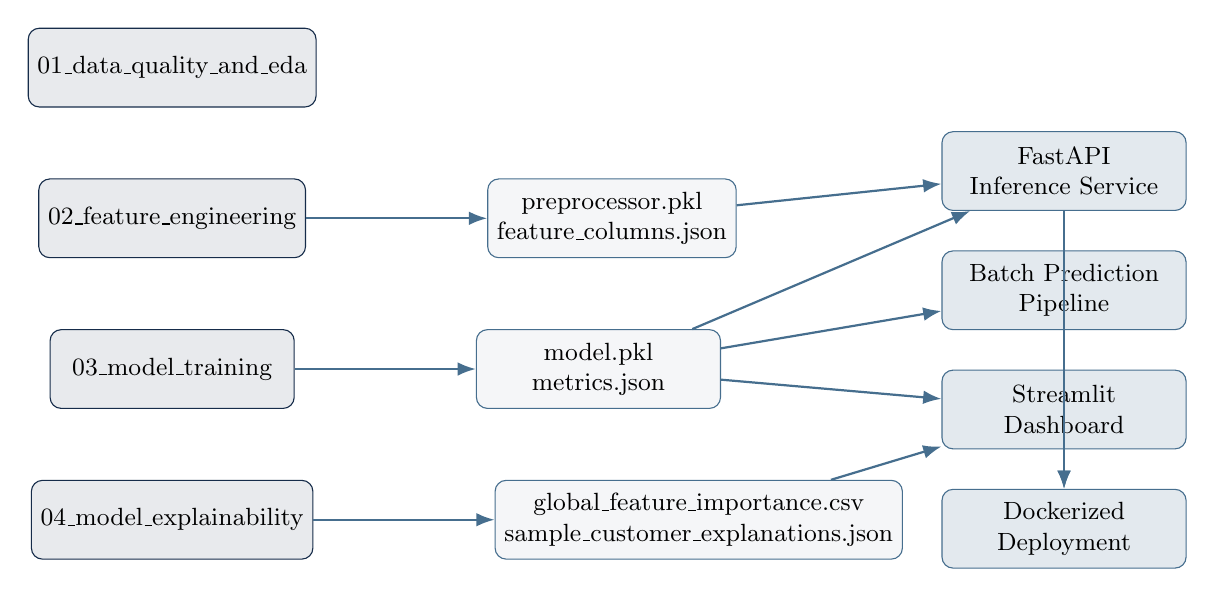
\begin{tikzpicture}[
    node distance=0.9cm and 1.6cm,
    box/.style={rectangle, rounded corners, draw=steel, fill=lightgray, minimum height=1cm, minimum width=3.1cm, align=center, font=\small},
    dsbox/.style={box, fill=navy!10, draw=navy},
    mlebox/.style={box, fill=steel!15, draw=steel},
    arr/.style={-Latex, thick, steel}
]

\node[dsbox] (nb01) {01\_data\_quality\_and\_eda};
\node[dsbox, below=of nb01] (nb02) {02\_feature\_engineering};
\node[dsbox, below=of nb02] (nb03) {03\_model\_training};
\node[dsbox, below=of nb03] (nb04) {04\_model\_explainability};

\node[box, right=2.3cm of nb02] (prep) {preprocessor.pkl \\ feature\_columns.json};
\node[box, right=2.3cm of nb03] (model) {model.pkl \\ metrics.json};
\node[box, right=2.3cm of nb04] (exp) {global\_feature\_importance.csv \\ sample\_customer\_explanations.json};

\draw[arr] (nb02) -- (prep);
\draw[arr] (nb03) -- (model);
\draw[arr] (nb04) -- (exp);

\node[mlebox, right=2.6cm of prep, yshift=0.6cm] (api) {FastAPI \\ Inference Service};
\node[mlebox, below=0.5cm of api] (batch) {Batch Prediction \\ Pipeline};
\node[mlebox, below=0.5cm of batch] (dash) {Streamlit \\ Dashboard};
\node[mlebox, below=0.5cm of dash] (docker) {Dockerized \\ Deployment};

\draw[arr] (prep) -- (api);
\draw[arr] (model) -- (api);
\draw[arr] (model) -- (batch);
\draw[arr] (exp) -- (dash);
\draw[arr] (model) -- (dash);
\draw[arr] (api) -- (docker);
\draw[arr] (batch) -- (docker);

\end{tikzpicture}
\caption{Artifact hand-off from the Data Science phase to the ML Engineering phase.}
\label{fig:handoff}
\end{figure}

\subsection{FastAPI Inference Pipeline}

The FastAPI service will load \artifact{model.pkl} once at process startup (not per-request, to avoid repeated deserialization latency). An incoming request's JSON body will first be validated against \artifact{feature\_columns.json}'s \texttt{raw\_input\_columns} list, then passed to \texttt{model.predict\_proba()}, which internally invokes the frozen preprocessing steps before the classifier. The response will include both the churn probability and, optionally, the top SHAP-driven features for that specific record --- computed on demand using the same \texttt{TreeExplainer} pattern established in Notebook 04, since \texttt{TreeExplainer} is cheap enough to run per-request rather than only in batch.

\subsection{Batch Prediction Pipeline}

The batch job will load the same \artifact{model.pkl}, read a dataframe of many customer records (retaining \artifact{customerID} alongside, per Section 2.1), call \texttt{model.predict\_proba()} once on the full batch for efficiency, and write back a probability column joined to the original identifiers. Because the preprocessing pipeline is embedded inside \artifact{model.pkl}, the batch job requires no separate cleaning logic of its own --- it is guaranteed to apply identical transformations to identical raw inputs as the FastAPI path, eliminating a common source of training/serving skew where batch and real-time paths drift apart over time.

\subsection{Streamlit Dashboard}

A dashboard consuming \artifact{metrics.json}, \artifact{global\_feature\_importance.csv}, and \artifact{sample\_customer\_explanations.json} can present the model's overall health (metrics over time, drift versus the recorded baseline) and let a retention agent explore an individual customer's SHAP-driven explanation interactively --- reusing the exact reasoning and artifact structure already established in Notebook 04, rather than recomputing explanations from scratch in a different codebase.

\subsection{Dockerized Deployment}

Because every artifact here is a plain file (pickle or JSON) with no dependency on the notebook execution environment itself, containerizing the inference service is a matter of packaging the artifacts, the \texttt{scikit-learn}/\texttt{xgboost}/\texttt{shap} runtime dependencies (versions pinned to match what produced these artifacts, to avoid pickle deserialization incompatibilities across library versions), and the FastAPI application code --- no notebook, and no access to the raw training CSV, is required inside the production container.

\subsection{How the Two Phases Connect}

The Data Science phase's central engineering contribution is not the model's accuracy number in isolation --- it is the fact that every transformation the model depends on was captured inside serializable, versionable artifacts, with an explicit, auditable feature contract (\artifact{feature\_columns.json}) and an explicit, auditable evaluation baseline (\artifact{metrics.json}). This is what allows the ML Engineering phase to build a service that does not need to re-derive, re-guess, or re-implement any cleaning or encoding logic --- it only needs to load four files and call well-defined interfaces on them.

% ======================================================================
\section{Lessons Learned}
% ======================================================================

\subsection{Key Technical Decisions Worth Remembering}

\begin{itemize}[leftmargin=1.4em]
    \item The \artifact{TotalCharges} blank-string issue was invisible to standard \texttt{isnull()} checks --- always inspect \texttt{dtype} mismatches (an \texttt{object} column that should be numeric) as a first-class data quality check, not an afterthought.
    \item Preprocessing must be built as a fittable, serializable \texttt{scikit-learn} object from the start of the project, not retrofitted later --- retrofitting risks subtle train/serve skew that is hard to detect after the fact.
    \item \texttt{handle\_unknown='ignore'} on the \texttt{OneHotEncoder} is a one-line change that prevents an entire class of future production outages; it is easy to overlook because it has zero effect on the current, static training/test data.
    \item Cross-validation must refit preprocessing per fold (via \texttt{clone(preprocessor)} inside each CV pipeline), not reuse one globally-fit preprocessor --- a leakage source that is easy to miss because it does not raise an error, only quietly inflates validation scores.
    \item Model selection criteria (ROC-AUC here) should be chosen to match how the model's output will actually be consumed downstream (a probability feeding a tiered recommendation engine), not defaulted to accuracy or F1 out of habit.
\end{itemize}

\subsection{Common Beginner Mistakes Avoided}

\begin{itemize}[leftmargin=1.4em]
    \item Trusting \texttt{df.isnull().sum() == 0} as proof of no missing data, without checking for disguised missingness (blank strings, sentinel values) in columns with an unexpected dtype.
    \item Fitting scalers/encoders on the full dataset before splitting into train/test (a leakage mistake that silently and consistently inflates reported model performance).
    \item Selecting a model purely by accuracy on an imbalanced target, which would have favored a near-trivial always-predict-majority-class model over any of the four candidates actually trained here.
    \item Treating SHAP-identified correlates (e.g., payment method) as causal levers for business action without stating the correlation-versus-causation caveat explicitly.
    \item Saving only a single combined artifact, which would have made it awkward for the explainability notebook to access transformed features and the raw classifier independently.
\end{itemize}

\subsection{Future Improvements}

\begin{enumerate}[leftmargin=1.4em]
    \item Calibrate the deployed decision threshold against actual retention-offer cost and customer lifetime value, rather than relying on the default 0.5 cutoff used for this phase's classification metrics.
    \item Incorporate behavioral/interaction-history features (support tickets, usage trend) if/when such data becomes available, since the current feature set is entirely static/account-level.
    \item Establish a production monitoring baseline directly from \artifact{metrics.json}, with automated drift/decay alerts and a defined retraining trigger.
    \item Consider segment-specific calibration (e.g., per contract type), given how strongly \artifact{Contract} interacts with other churn drivers in both the EDA and the SHAP analysis.
    \item Run a controlled experiment (A/B test) on the eventual recommendation engine's actions themselves, not just the underlying model's offline metrics, to confirm the SHAP-informed interventions actually reduce real-world churn.
\end{enumerate}

\end{document}